\documentclass{standalone}
\usepackage{tikz}
\usetikzlibrary{patterns, positioning}


\begin{document}
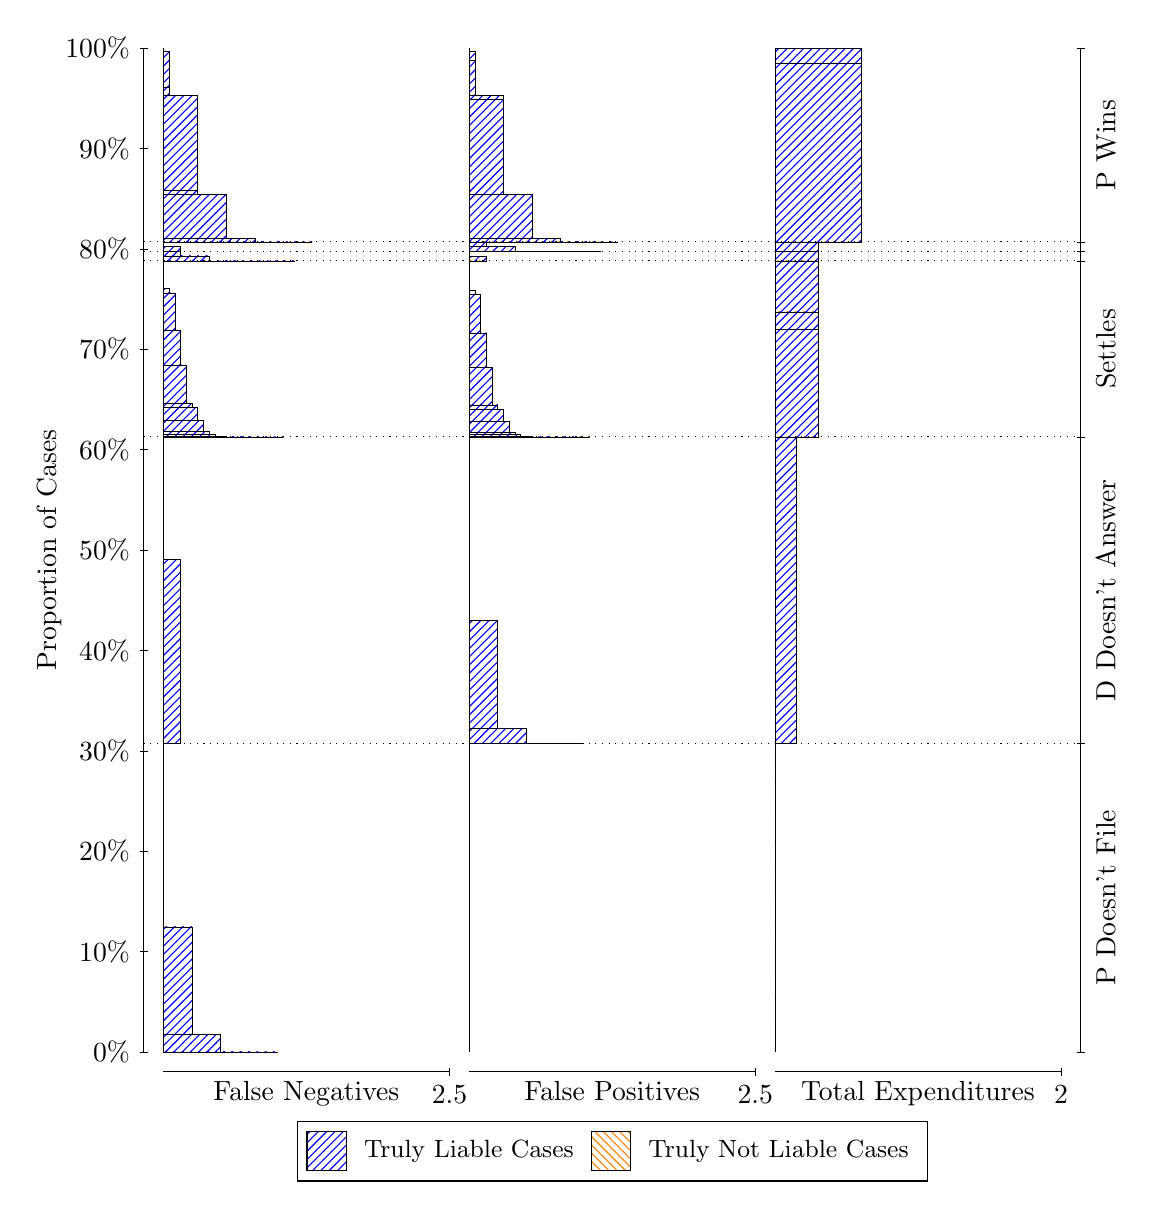
\begin{tikzpicture}
\draw[black, very thin] (1.5,1.75) -- (1.5,14.5);
\node[rotate=90, text=black, anchor=center] at (0.3, 8.125) {Proportion of Cases};
\draw[black, very thin] (1.45,1.75) -- (1.55,1.75);
\node[text=black, anchor=east] at (1.45, 1.75) {0\%};
\draw[black, very thin] (1.45,3.025) -- (1.55,3.025);
\node[text=black, anchor=east] at (1.45, 3.025) {10\%};
\draw[black, very thin] (1.45,4.3) -- (1.55,4.3);
\node[text=black, anchor=east] at (1.45, 4.3) {20\%};
\draw[black, very thin] (1.45,5.575) -- (1.55,5.575);
\node[text=black, anchor=east] at (1.45, 5.575) {30\%};
\draw[black, very thin] (1.45,6.85) -- (1.55,6.85);
\node[text=black, anchor=east] at (1.45, 6.85) {40\%};
\draw[black, very thin] (1.45,8.125) -- (1.55,8.125);
\node[text=black, anchor=east] at (1.45, 8.125) {50\%};
\draw[black, very thin] (1.45,9.4) -- (1.55,9.4);
\node[text=black, anchor=east] at (1.45, 9.4) {60\%};
\draw[black, very thin] (1.45,10.675) -- (1.55,10.675);
\node[text=black, anchor=east] at (1.45, 10.675) {70\%};
\draw[black, very thin] (1.45,11.95) -- (1.55,11.95);
\node[text=black, anchor=east] at (1.45, 11.95) {80\%};
\draw[black, very thin] (1.45,13.225) -- (1.55,13.225);
\node[text=black, anchor=east] at (1.45, 13.225) {90\%};
\draw[black, very thin] (1.45,14.5) -- (1.55,14.5);
\node[text=black, anchor=east] at (1.45, 14.5) {100\%};

\draw[black, very thin] (13.4,1.75) -- (13.4,14.5);
\draw[black, very thin] (13.35,1.75) -- (13.45,1.75);
\node[anchor=west] at (13.35, 1.75) {};
\draw[black, very thin] (13.35,5.6692) -- (13.45,5.6692);
\node[anchor=west] at (13.35, 5.6692) {};
\draw[black, very thin] (13.35,9.5618) -- (13.45,9.5618);
\node[anchor=west] at (13.35, 9.5618) {};
\draw[black, very thin] (13.35,11.796) -- (13.45,11.796);
\node[anchor=west] at (13.35, 11.796) {};
\draw[black, very thin] (13.35,11.917) -- (13.45,11.917);
\node[anchor=west] at (13.35, 11.917) {};
\draw[black, very thin] (13.35,12.038) -- (13.45,12.038);
\node[anchor=west] at (13.35, 12.038) {};
\draw[black, very thin] (13.35,14.5) -- (13.45,14.5);
\node[anchor=west] at (13.35, 14.5) {};

\draw[black, very thin, pattern color=blue, pattern=north east lines] (1.75,1.75) rectangle (3.2033,1.75);
\draw[black, very thin, pattern color=blue, pattern=north east lines] (1.75,1.75) rectangle (2.84,1.7519);
\draw[black, very thin, pattern color=blue, pattern=north east lines] (1.75,1.7519) rectangle (2.4767,1.9762);
\draw[black, very thin, pattern color=blue, pattern=north east lines] (1.75,1.9762) rectangle (2.1133,3.3375);
\draw[black, very thin, pattern color=orange, pattern=north west lines] (1.75,3.3375) rectangle (1.75,3.3375);
\draw[black, very thin, pattern color=blue, pattern=north east lines] (1.75,3.3375) rectangle (1.75,5.6692);
\draw[black, very thin, pattern color=blue, pattern=north east lines] (1.75,5.6692) rectangle (1.968,8.002);
\draw[black, very thin, pattern color=orange, pattern=north west lines] (1.75,8.002) rectangle (1.75,8.002);
\draw[black, very thin, pattern color=blue, pattern=north east lines] (1.75,8.002) rectangle (1.75,9.5618);
\draw[black, very thin, pattern color=blue, pattern=north east lines] (1.75,9.5618) rectangle (3.276,9.5618);
\draw[black, very thin, pattern color=blue, pattern=north east lines] (1.75,9.5618) rectangle (2.9853,9.5618);
\draw[black, very thin, pattern color=blue, pattern=north east lines] (1.75,9.5618) rectangle (2.9127,9.5618);
\draw[black, very thin, pattern color=blue, pattern=north east lines] (1.75,9.5618) rectangle (2.6947,9.5619);
\draw[black, very thin, pattern color=blue, pattern=north east lines] (1.75,9.5619) rectangle (2.622,9.5621);
\draw[black, very thin, pattern color=blue, pattern=north east lines] (1.75,9.5621) rectangle (2.5493,9.5692);
\draw[black, very thin, pattern color=blue, pattern=north east lines] (1.75,9.5692) rectangle (2.404,9.5969);
\draw[black, very thin, pattern color=blue, pattern=north east lines] (1.75,9.5969) rectangle (2.3313,9.6294);
\draw[black, very thin, pattern color=blue, pattern=north east lines] (1.75,9.6294) rectangle (2.2587,9.7713);
\draw[black, very thin, pattern color=blue, pattern=north east lines] (1.75,9.7713) rectangle (2.186,9.9362);
\draw[black, very thin, pattern color=blue, pattern=north east lines] (1.75,9.9362) rectangle (2.1133,9.989);
\draw[black, very thin, pattern color=blue, pattern=north east lines] (1.75,9.989) rectangle (2.0407,10.477);
\draw[black, very thin, pattern color=blue, pattern=north east lines] (1.75,10.477) rectangle (1.968,10.911);
\draw[black, very thin, pattern color=blue, pattern=north east lines] (1.75,10.911) rectangle (1.8953,11.39);
\draw[black, very thin, pattern color=blue, pattern=north east lines] (1.75,11.39) rectangle (1.8227,11.445);
\draw[black, very thin, pattern color=orange, pattern=north west lines] (1.75,11.445) rectangle (1.75,11.445);
\draw[black, very thin, pattern color=blue, pattern=north east lines] (1.75,11.445) rectangle (1.75,11.796);
\draw[black, very thin, pattern color=blue, pattern=north east lines] (1.75,11.796) rectangle (3.4213,11.796);
\draw[black, very thin, pattern color=blue, pattern=north east lines] (1.75,11.796) rectangle (3.058,11.796);
\draw[black, very thin, pattern color=blue, pattern=north east lines] (1.75,11.796) rectangle (2.6947,11.798);
\draw[black, very thin, pattern color=blue, pattern=north east lines] (1.75,11.798) rectangle (2.3313,11.859);
\draw[black, very thin, pattern color=blue, pattern=north east lines] (1.75,11.859) rectangle (1.968,11.917);
\draw[black, very thin, pattern color=orange, pattern=north west lines] (1.75,11.917) rectangle (1.75,11.917);
\draw[black, very thin, pattern color=blue, pattern=north east lines] (1.75,11.917) rectangle (1.968,11.976);
\draw[black, very thin, pattern color=orange, pattern=north west lines] (1.75,11.976) rectangle (1.75,11.976);
\draw[black, very thin, pattern color=blue, pattern=north east lines] (1.75,11.976) rectangle (1.75,12.038);
\draw[black, very thin, pattern color=blue, pattern=north east lines] (1.75,12.038) rectangle (3.6393,12.038);
\draw[black, very thin, pattern color=blue, pattern=north east lines] (1.75,12.038) rectangle (3.276,12.038);
\draw[black, very thin, pattern color=blue, pattern=north east lines] (1.75,12.038) rectangle (2.9127,12.082);
\draw[black, very thin, pattern color=blue, pattern=north east lines] (1.75,12.082) rectangle (2.5493,12.641);
\draw[black, very thin, pattern color=blue, pattern=north east lines] (1.75,12.641) rectangle (2.186,12.693);
\draw[black, very thin, pattern color=blue, pattern=north east lines] (1.75,12.693) rectangle (2.186,13.897);
\draw[black, very thin, pattern color=blue, pattern=north east lines] (1.75,13.897) rectangle (1.8227,14.003);
\draw[black, very thin, pattern color=blue, pattern=north east lines] (1.75,14.003) rectangle (1.8227,14.456);
\draw[black, very thin, pattern color=orange, pattern=north west lines] (1.75,14.456) rectangle (1.75,14.456);
\draw[black, very thin, pattern color=blue, pattern=north east lines] (1.75,14.456) rectangle (1.75,14.5);
\draw[black, very thin, pattern color=orange, pattern=north west lines] (5.6333,1.75) rectangle (5.6333,1.75);
\draw[black, very thin, pattern color=blue, pattern=north east lines] (5.6333,1.75) rectangle (5.6333,5.6692);
\draw[black, very thin, pattern color=orange, pattern=north west lines] (5.6333,5.6692) rectangle (7.0867,5.6692);
\draw[black, very thin, pattern color=blue, pattern=north east lines] (5.6333,5.6692) rectangle (7.0867,5.6692);
\draw[black, very thin, pattern color=blue, pattern=north east lines] (5.6333,5.6692) rectangle (6.7233,5.6696);
\draw[black, very thin, pattern color=blue, pattern=north east lines] (5.6333,5.6696) rectangle (6.36,5.8643);
\draw[black, very thin, pattern color=blue, pattern=north east lines] (5.6333,5.8643) rectangle (5.9967,7.229);
\draw[black, very thin, pattern color=blue, pattern=north east lines] (5.6333,7.229) rectangle (5.6333,9.5618);
\draw[black, very thin, pattern color=orange, pattern=north west lines] (5.6333,9.5618) rectangle (7.1593,9.5618);
\draw[black, very thin, pattern color=blue, pattern=north east lines] (5.6333,9.5618) rectangle (7.1593,9.5618);
\draw[black, very thin, pattern color=orange, pattern=north west lines] (5.6333,9.5618) rectangle (6.8687,9.5618);
\draw[black, very thin, pattern color=blue, pattern=north east lines] (5.6333,9.5618) rectangle (6.8687,9.5618);
\draw[black, very thin, pattern color=blue, pattern=north east lines] (5.6333,9.5618) rectangle (6.796,9.5618);
\draw[black, very thin, pattern color=orange, pattern=north west lines] (5.6333,9.5618) rectangle (6.578,9.5618);
\draw[black, very thin, pattern color=blue, pattern=north east lines] (5.6333,9.5618) rectangle (6.578,9.5618);
\draw[black, very thin, pattern color=blue, pattern=north east lines] (5.6333,9.5618) rectangle (6.5053,9.5621);
\draw[black, very thin, pattern color=blue, pattern=north east lines] (5.6333,9.5621) rectangle (6.4327,9.5685);
\draw[black, very thin, pattern color=orange, pattern=north west lines] (5.6333,9.5685) rectangle (6.2873,9.5685);
\draw[black, very thin, pattern color=blue, pattern=north east lines] (5.6333,9.5685) rectangle (6.2873,9.5954);
\draw[black, very thin, pattern color=blue, pattern=north east lines] (5.6333,9.5954) rectangle (6.2147,9.621);
\draw[black, very thin, pattern color=blue, pattern=north east lines] (5.6333,9.621) rectangle (6.142,9.7627);
\draw[black, very thin, pattern color=blue, pattern=north east lines] (5.6333,9.7627) rectangle (6.0693,9.9134);
\draw[black, very thin, pattern color=orange, pattern=north west lines] (5.6333,9.9134) rectangle (5.9967,9.9134);
\draw[black, very thin, pattern color=blue, pattern=north east lines] (5.6333,9.9134) rectangle (5.9967,9.9683);
\draw[black, very thin, pattern color=blue, pattern=north east lines] (5.6333,9.9683) rectangle (5.924,10.447);
\draw[black, very thin, pattern color=blue, pattern=north east lines] (5.6333,10.447) rectangle (5.8513,10.881);
\draw[black, very thin, pattern color=blue, pattern=north east lines] (5.6333,10.881) rectangle (5.7787,11.369);
\draw[black, very thin, pattern color=blue, pattern=north east lines] (5.6333,11.369) rectangle (5.706,11.422);
\draw[black, very thin, pattern color=blue, pattern=north east lines] (5.6333,11.422) rectangle (5.6333,11.796);
\draw[black, very thin, pattern color=orange, pattern=north west lines] (5.6333,11.796) rectangle (5.8513,11.796);
\draw[black, very thin, pattern color=blue, pattern=north east lines] (5.6333,11.796) rectangle (5.8513,11.855);
\draw[black, very thin, pattern color=blue, pattern=north east lines] (5.6333,11.855) rectangle (5.6333,11.917);
\draw[black, very thin, pattern color=orange, pattern=north west lines] (5.6333,11.917) rectangle (7.3047,11.917);
\draw[black, very thin, pattern color=blue, pattern=north east lines] (5.6333,11.917) rectangle (7.3047,11.917);
\draw[black, very thin, pattern color=blue, pattern=north east lines] (5.6333,11.917) rectangle (6.9413,11.917);
\draw[black, very thin, pattern color=blue, pattern=north east lines] (5.6333,11.917) rectangle (6.578,11.919);
\draw[black, very thin, pattern color=blue, pattern=north east lines] (5.6333,11.919) rectangle (6.2147,11.98);
\draw[black, very thin, pattern color=blue, pattern=north east lines] (5.6333,11.98) rectangle (5.8513,12.038);
\draw[black, very thin, pattern color=orange, pattern=north west lines] (5.6333,12.038) rectangle (7.5227,12.038);
\draw[black, very thin, pattern color=blue, pattern=north east lines] (5.6333,12.038) rectangle (7.5227,12.038);
\draw[black, very thin, pattern color=orange, pattern=north west lines] (5.6333,12.038) rectangle (7.1593,12.038);
\draw[black, very thin, pattern color=blue, pattern=north east lines] (5.6333,12.038) rectangle (7.1593,12.038);
\draw[black, very thin, pattern color=orange, pattern=north west lines] (5.6333,12.038) rectangle (6.796,12.038);
\draw[black, very thin, pattern color=blue, pattern=north east lines] (5.6333,12.038) rectangle (6.796,12.082);
\draw[black, very thin, pattern color=orange, pattern=north west lines] (5.6333,12.082) rectangle (6.4327,12.082);
\draw[black, very thin, pattern color=blue, pattern=north east lines] (5.6333,12.082) rectangle (6.4327,12.641);
\draw[black, very thin, pattern color=blue, pattern=north east lines] (5.6333,12.641) rectangle (6.0693,13.845);
\draw[black, very thin, pattern color=orange, pattern=north west lines] (5.6333,13.845) rectangle (6.0693,13.845);
\draw[black, very thin, pattern color=blue, pattern=north east lines] (5.6333,13.845) rectangle (6.0693,13.897);
\draw[black, very thin, pattern color=blue, pattern=north east lines] (5.6333,13.897) rectangle (5.706,14.348);
\draw[black, very thin, pattern color=blue, pattern=north east lines] (5.6333,14.348) rectangle (5.706,14.456);
\draw[black, very thin, pattern color=blue, pattern=north east lines] (5.6333,14.456) rectangle (5.6333,14.5);
\draw[black, very thin, pattern color=orange, pattern=north west lines] (9.5167,1.75) rectangle (9.5167,1.75);
\draw[black, very thin, pattern color=blue, pattern=north east lines] (9.5167,1.75) rectangle (9.5167,5.6692);
\draw[black, very thin, pattern color=orange, pattern=north west lines] (9.5167,5.6692) rectangle (9.7892,5.6692);
\draw[black, very thin, pattern color=blue, pattern=north east lines] (9.5167,5.6692) rectangle (9.7892,9.5618);
\draw[black, very thin, pattern color=orange, pattern=north west lines] (9.5167,9.5618) rectangle (10.062,9.5618);
\draw[black, very thin, pattern color=blue, pattern=north east lines] (9.5167,9.5618) rectangle (10.062,10.922);
\draw[black, very thin, pattern color=orange, pattern=north west lines] (9.5167,10.922) rectangle (10.062,10.922);
\draw[black, very thin, pattern color=blue, pattern=north east lines] (9.5167,10.922) rectangle (10.062,11.149);
\draw[black, very thin, pattern color=orange, pattern=north west lines] (9.5167,11.149) rectangle (10.062,11.149);
\draw[black, very thin, pattern color=blue, pattern=north east lines] (9.5167,11.149) rectangle (10.062,11.796);
\draw[black, very thin, pattern color=orange, pattern=north west lines] (9.5167,11.796) rectangle (10.062,11.796);
\draw[black, very thin, pattern color=blue, pattern=north east lines] (9.5167,11.796) rectangle (10.062,11.917);
\draw[black, very thin, pattern color=orange, pattern=north west lines] (9.5167,11.917) rectangle (10.062,11.917);
\draw[black, very thin, pattern color=blue, pattern=north east lines] (9.5167,11.917) rectangle (10.062,12.038);
\draw[black, very thin, pattern color=orange, pattern=north west lines] (9.5167,12.038) rectangle (10.607,12.038);
\draw[black, very thin, pattern color=blue, pattern=north east lines] (9.5167,12.038) rectangle (10.607,14.309);
\draw[black, very thin, pattern color=orange, pattern=north west lines] (9.5167,14.309) rectangle (10.607,14.309);
\draw[black, very thin, pattern color=blue, pattern=north east lines] (9.5167,14.309) rectangle (10.607,14.5);
\draw[black, dotted] (1.5,5.6692) -- (13.4,5.6692);
\draw[black, dotted] (1.5,9.5618) -- (13.4,9.5618);
\draw[black, dotted] (1.5,11.796) -- (13.4,11.796);
\draw[black, dotted] (1.5,11.917) -- (13.4,11.917);
\draw[black, dotted] (1.5,12.038) -- (13.4,12.038);
\draw[black, very thin] (1.75,1.5) -- (5.3833,1.5);
\node[text=black, anchor=north] at (3.5667, 1.5) {False Negatives};
\draw[black, very thin] (5.3833,1.45) -- (5.3833,1.55);
\node[text=black, anchor=north] at (5.3833, 1.45) {2.5};

\draw[black, very thin] (5.6333,1.5) -- (9.2667,1.5);
\node[text=black, anchor=north] at (7.45, 1.5) {False Positives};
\draw[black, very thin] (9.2667,1.45) -- (9.2667,1.55);
\node[text=black, anchor=north] at (9.2667, 1.45) {2.5};

\draw[black, very thin] (9.5167,1.5) -- (13.15,1.5);
\node[text=black, anchor=north] at (11.333, 1.5) {Total Expenditures};
\draw[black, very thin] (13.15,1.45) -- (13.15,1.55);
\node[text=black, anchor=north] at (13.15, 1.45) {2};

\node[text=black, centered, rotate=90] at (13.72, 3.7096) {P Doesn't File};
\node[text=black, centered, rotate=90] at (13.72, 7.6155) {D Doesn't Answer};
\node[text=black, centered, rotate=90] at (13.72, 10.679) {Settles};


\node[text=black, centered, rotate=90] at (13.72, 13.269) {P Wins};

\draw (7.449999999999999,1.5) node[draw=none] (baseCoordinate) {};
\begin{scope}[align=center]
        \matrix[scale=0.5, draw=black, below=0.5cm of baseCoordinate, nodes={draw}, column sep=0.1cm]{
            \node[rectangle, draw, minimum width=0.5cm, minimum height=0.5cm, pattern color=blue, pattern=north east lines] {}; &
            \node[draw=none, font=\small, text=black] (B) {Truly Liable Cases}; &
            \node[rectangle, draw, minimum width=0.5cm, minimum height=0.5cm, pattern color=orange, pattern=north west lines] {}; &
            \node[draw=none, font=\small, text=black] (B) {Truly Not Liable Cases}; \\
            };
\end{scope}

\end{tikzpicture}
\end{document}